\chapter{C++ Packages}\label{chap6}
\section{Pythia, FastJet and ROOT}
Pythia is a general-purpose event generator. It is extensively used for studying physics at LHC. At the beginning the code was written in \verb+Fortran 77+, recently it has been moved to \verb!C++!. The latest version of Pythia (8.1) was released in 2007, which is written in \verb!C++!  \citep{Buckley:2011ms}.
%\Jnote{C++ with capital letter.}

In general Pythia performs a similar simulations as our model of the parton shower.
%\Jnote{Rephrase: ``...performs similar simulations as our model of the parton
%  shower.''}
However, it accounts for more of the underlying physics,that we have not covered in our model. Such  as the quark flavour or in general the type of the particle which is splitting.  


\verb+FastJet+ is an analysis tools, it written in \verb!C++!. It includes efficient implementation of all widely used sequential recombination jet algorithms. In the case of jet clustering, the working principle is the same as the algorithm that we implemented in chapter \ref{chapter4},
%\Jnote{Do not reference chapters by hand.}
but it is much faster \citep{Buckley:2011ms}. 

\verb+ROOT+ is a scientific software library that provides a wide range of tools that can be used for big data processing. \verb+ROOT+ provides a histogrammming packages (which we used), as well as graphing. This alongside with other features concerning data analysis.  
\section{Our Simulation}
In our work we generated 1000 events using Pythia 8.1 and analysed them using \verb+FastJet+ using the configuration $dijet$, which is the a simulation of a collision that produces two particles. First two protons will collide and we focus on three types of  interactions, quark gluon produces quark gluon, two quarks produces two quarks and quark anti quark produces two gluons.    

We extracted the same  observables as in \ref{nofcon}, \ref{nofjet} and \ref{pseudomass}  the pseudo-mass, the number of constituents in the jet with highest energy and the number of jet observables, and using \verb+ROOT+ we produced histograms of these observables. In this analysis the value of the parameter $R$ is set to 1.

The \verb!C++! code that we used in this work is based on the code shared with us form Samuel Meheen and it is available on \url{https://github.com/smeehan12/PythiaSimulatorAnalysis} 
%\Jnote{Consider different sections: For example: Chapter ``C++ Packages'',
%  one section describing Pythia + FastJet + Root, another section
%  summarizing your simulation.}

\begin{figure}[hbtp]
\centering
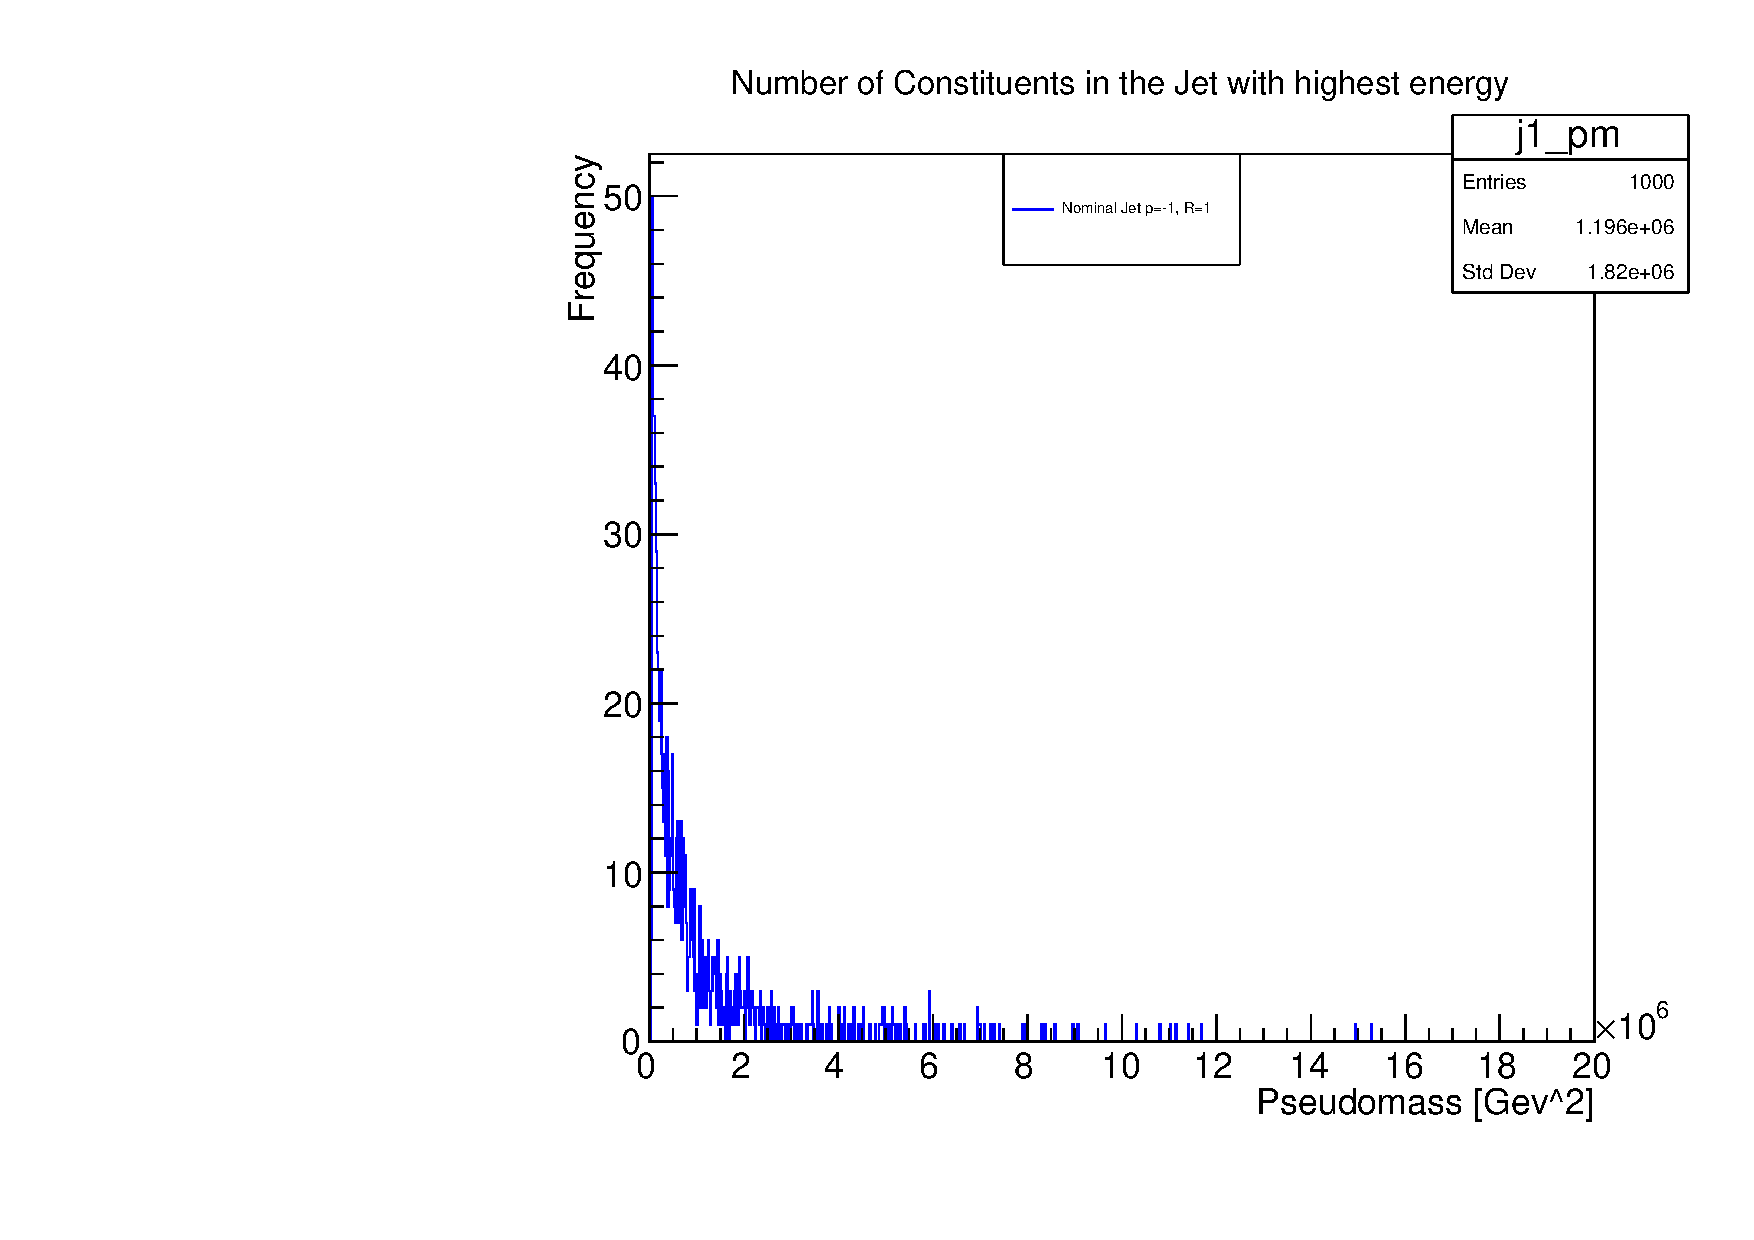
\includegraphics[scale=.7]{images/myplot1.pdf}
\caption{A histogram of the pseudo-mass of a jet observable obtained from analysing 1000 events. $R$ is chosen to be 1.}
\end{figure}



\begin{figure}[hbtp]
\centering
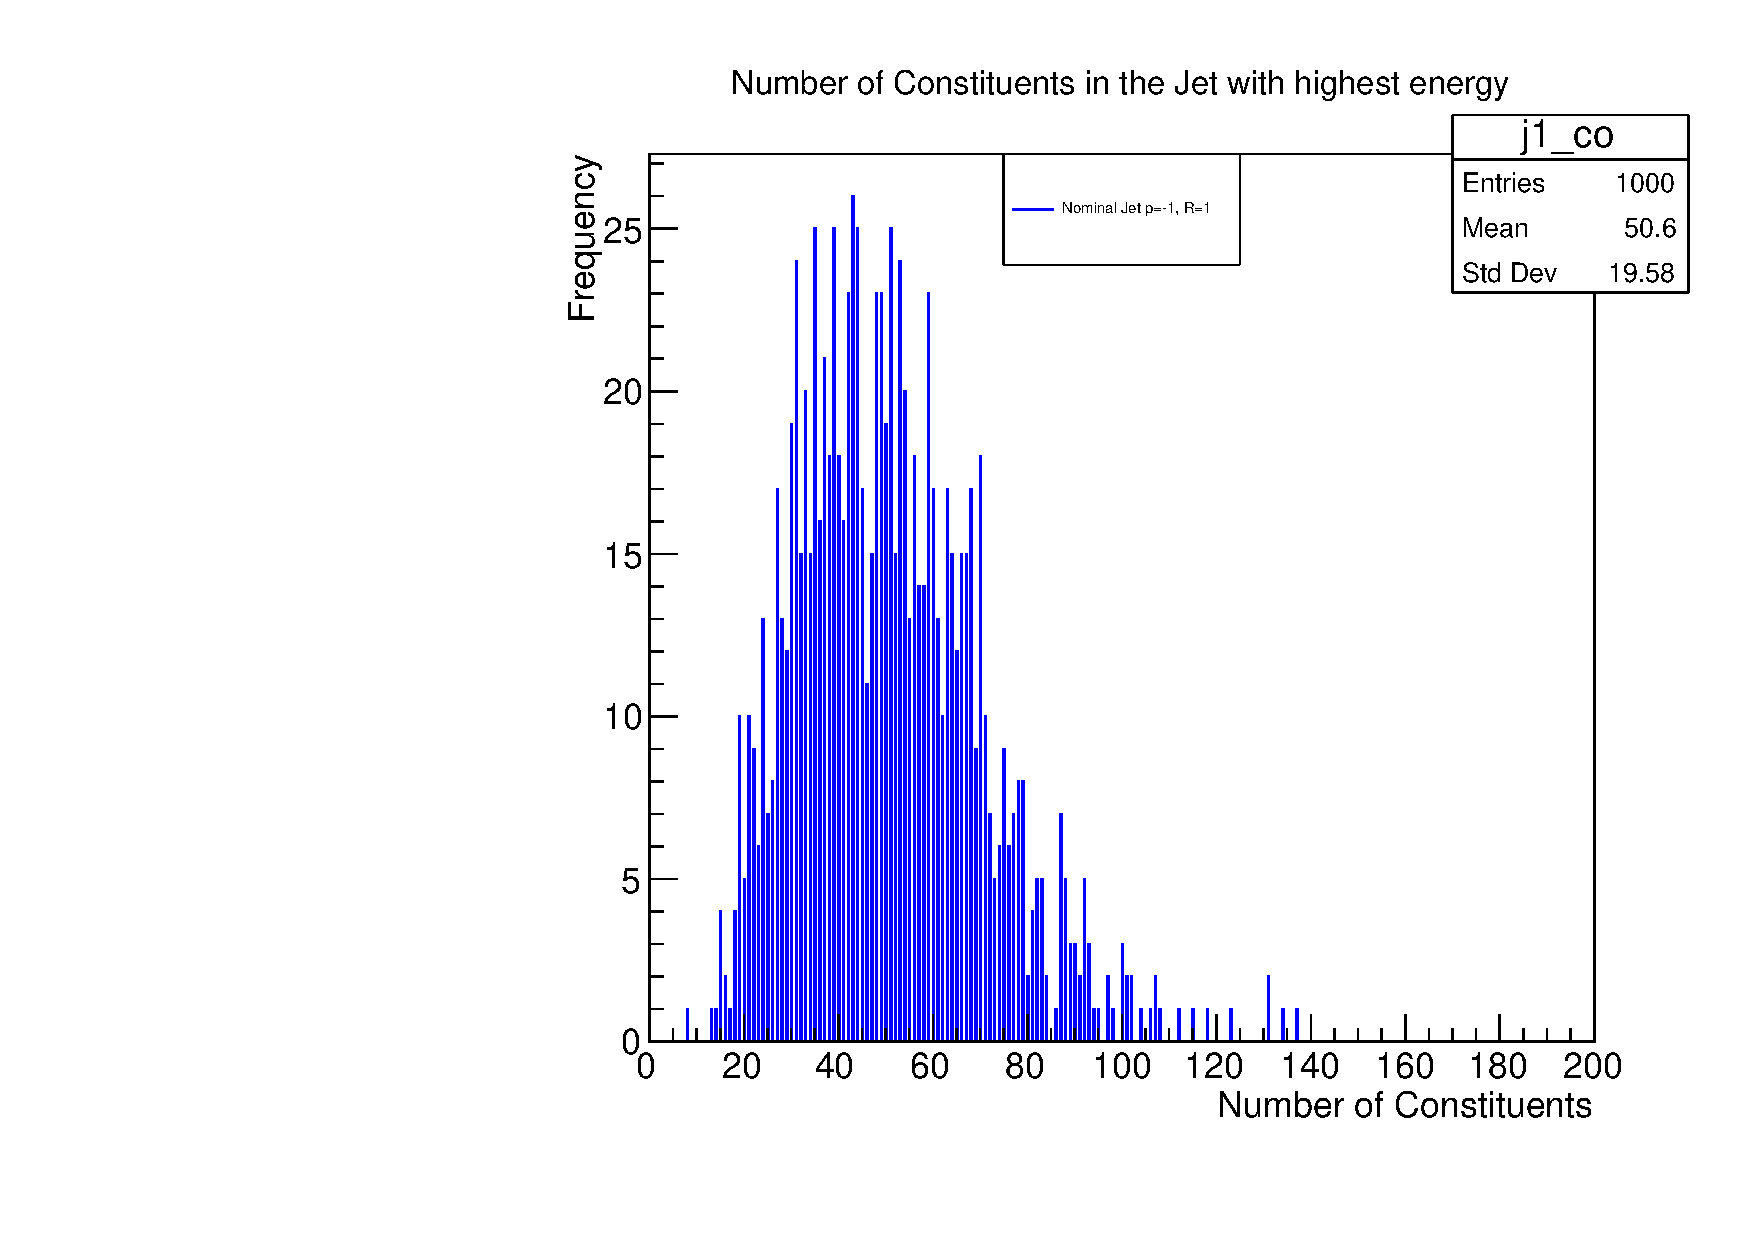
\includegraphics[scale=.7]{images/myplot3.pdf}
\caption{A histogram of the number of constituents in the jet with highest energy obtained from analysing 1000 events.}
\end{figure}

 
\begin{figure}[hbtp]
\centering
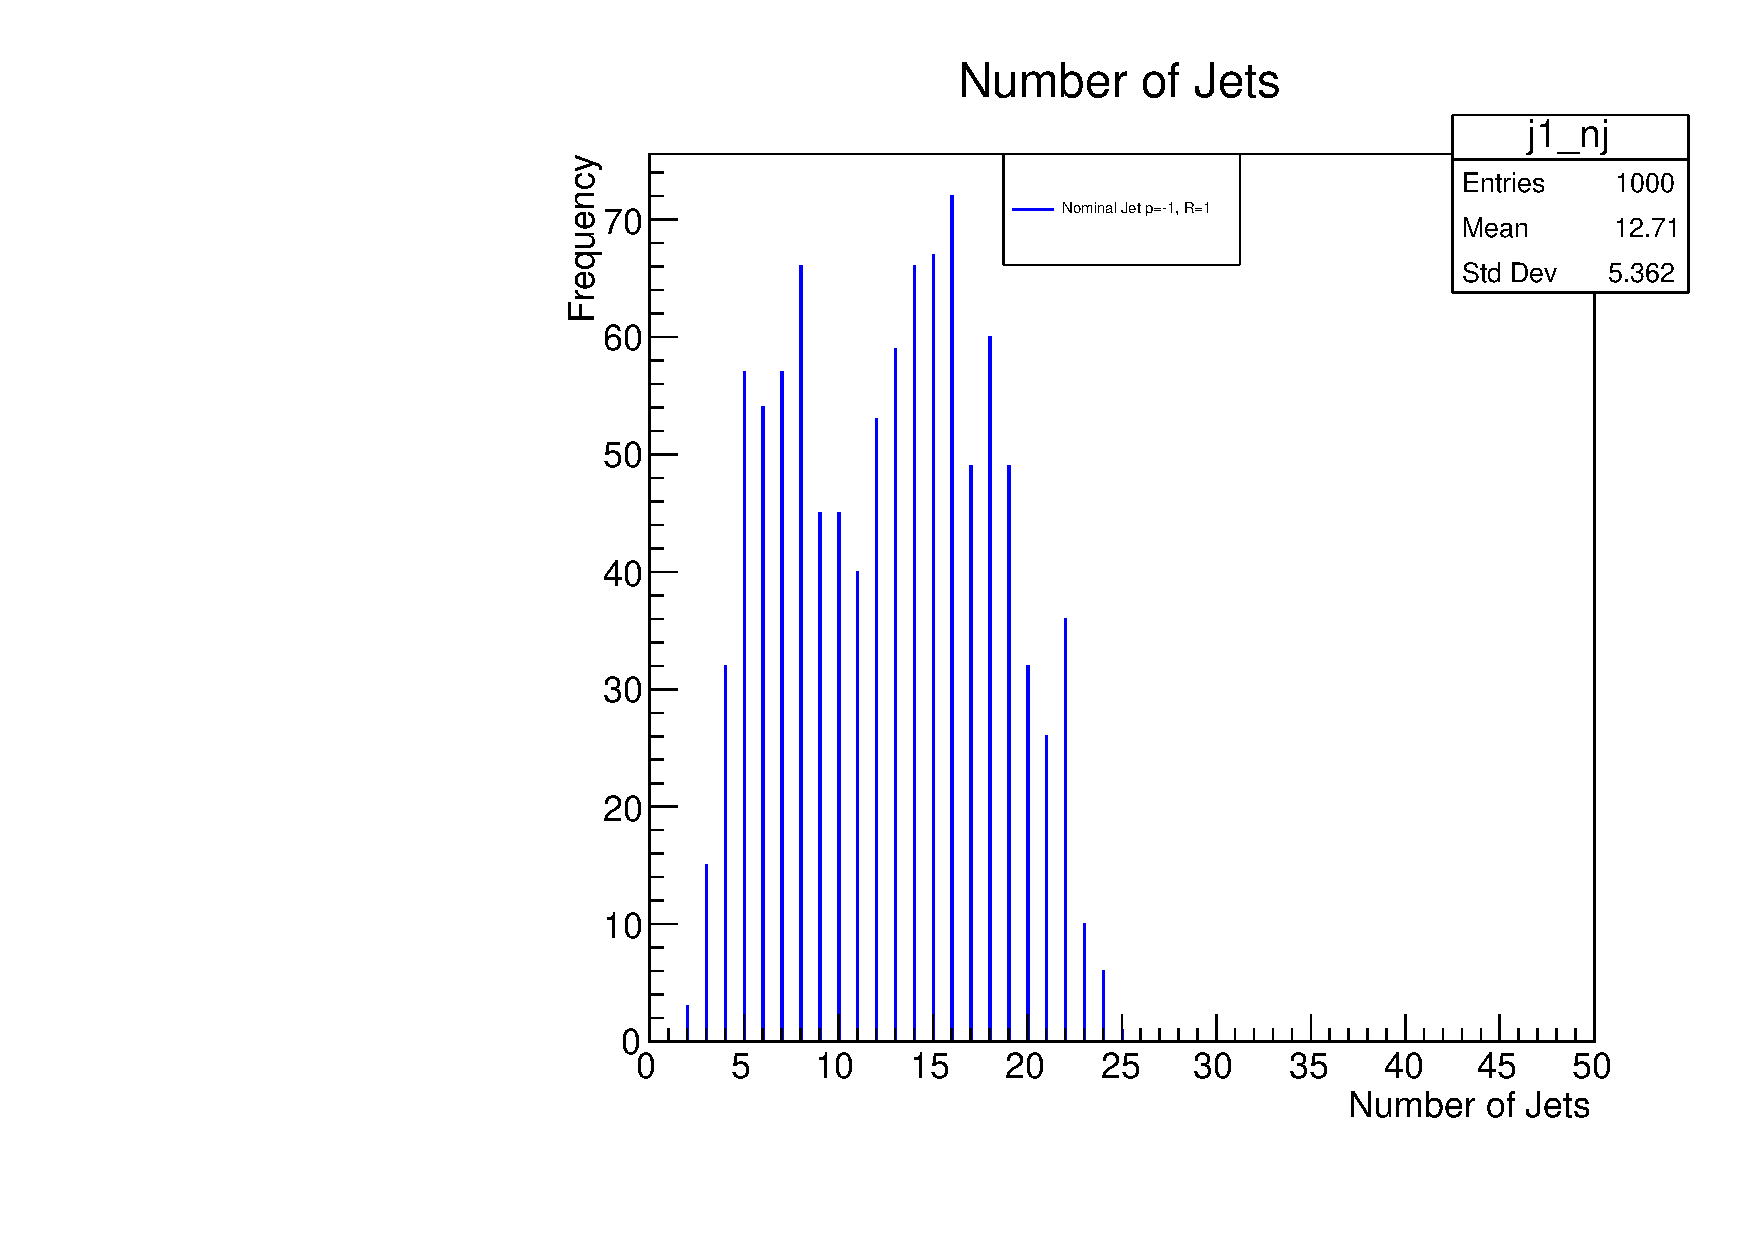
\includegraphics[scale=.7]{images/myplot2.pdf}
\caption{A histogram of the number of jet obtained analysing from 1000 events.}
\end{figure}

%\begin{figure}[hbtp]
%\centering
%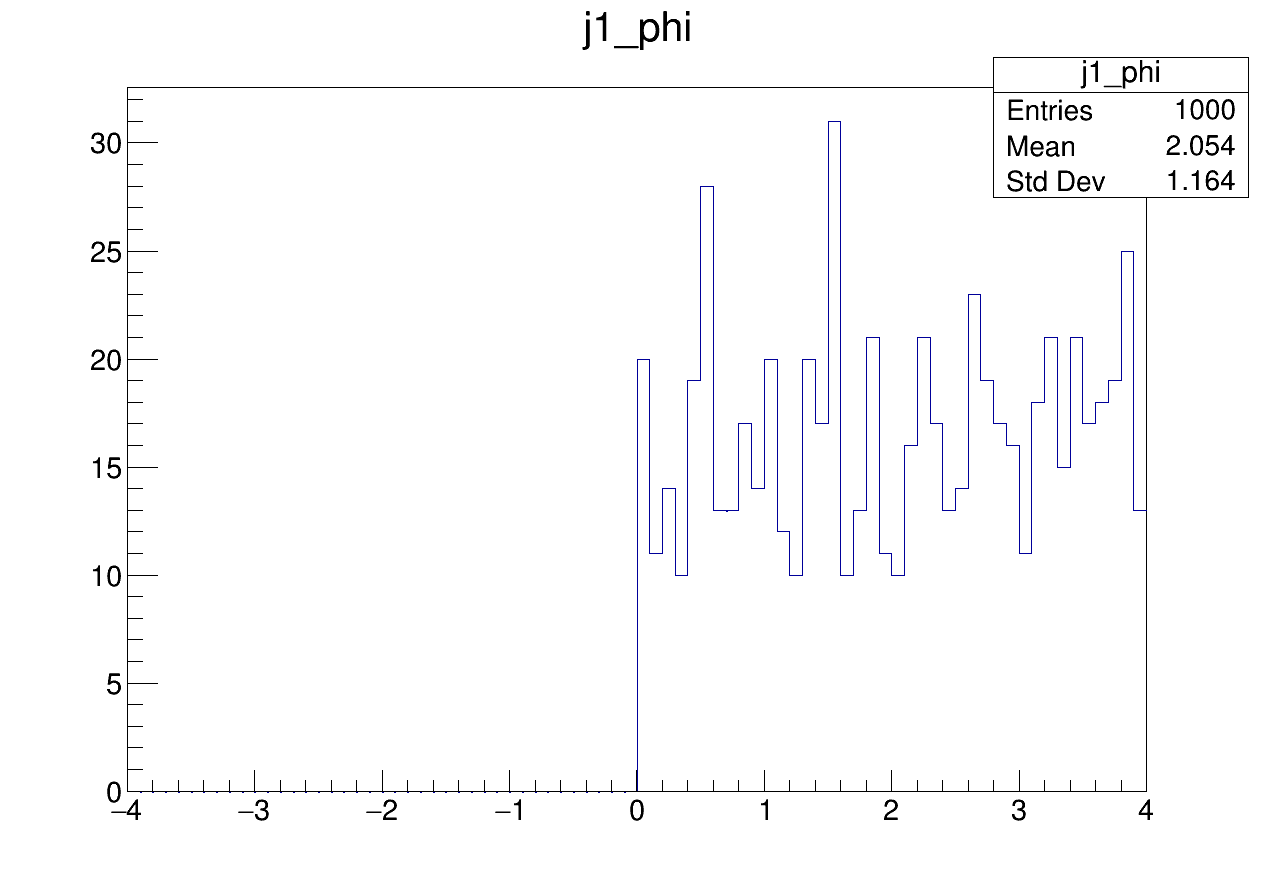
\includegraphics[scale=.4]{images/phi.png}
%\caption{The Azimuth distance.  }
%\end{figure}
%
%\begin{figure}[hbtp]
%\centering
%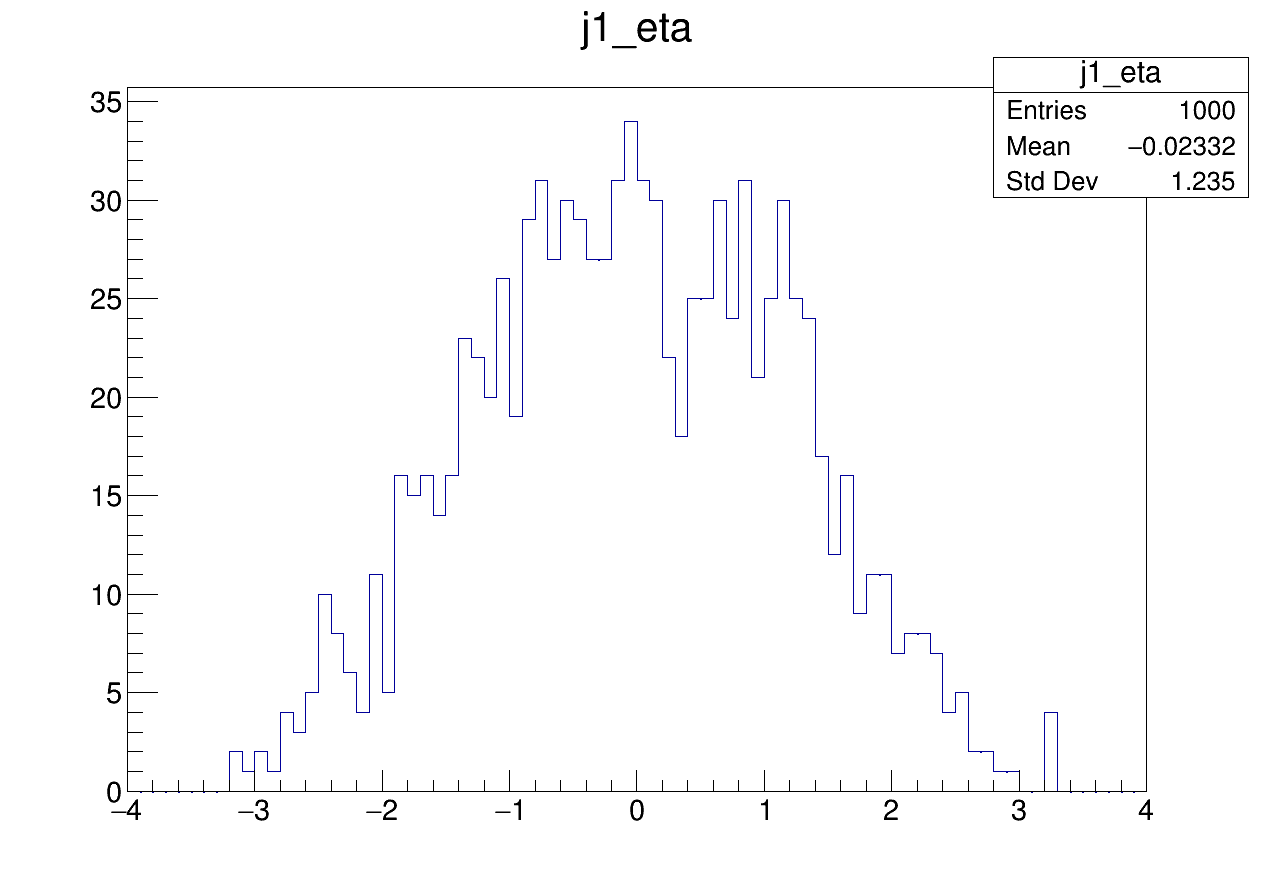
\includegraphics[scale=.3]{images/eta.png}
%\caption{The pseudo-rapidity}
%\end{figure}    